\begin{figure}[!htb]
	\centering
	\begin{subfigure}{0.48\linewidth}
		\centering
		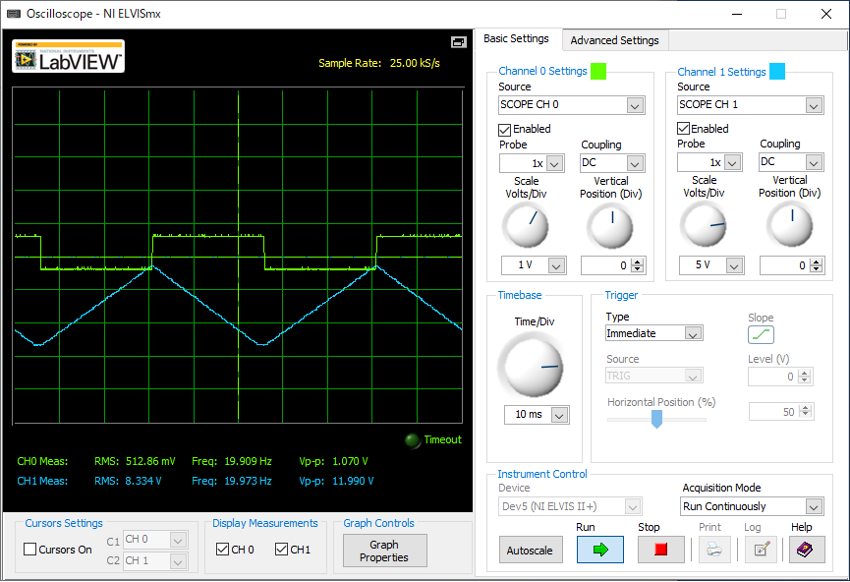
\includegraphics[width=0.8\linewidth]{src/figures/exp6/int.png}
		\subcaption{積分回路に矩形波を入力した時の出力}\label{fig:exp6-int}
	\end{subfigure}
	\begin{subfigure}{0.48\linewidth}
		\centering
		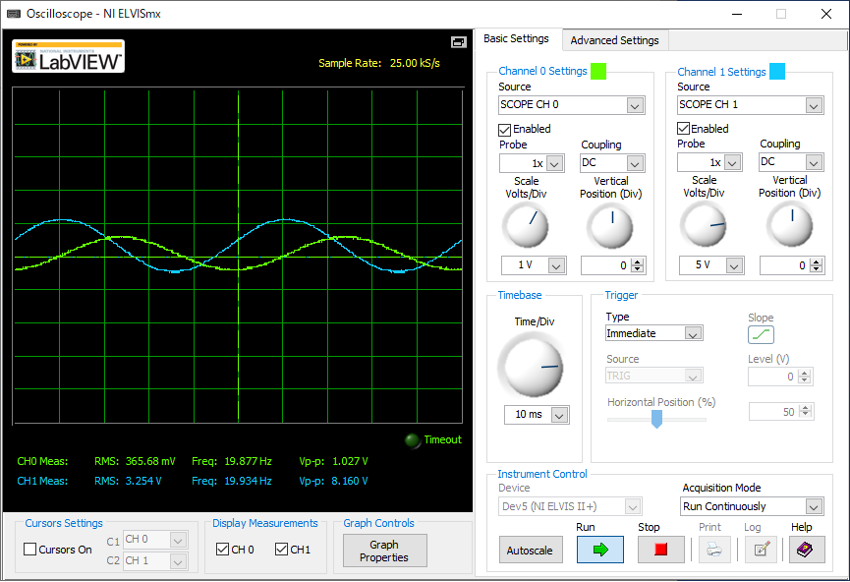
\includegraphics[width=0.8\linewidth]{src/figures/exp6/int-res-sin.png}
		\subcaption{不完全積分回路に正弦波を入力したときの出力}\label{fig:exp6-int-res-sin}
	\end{subfigure}
	\begin{subfigure}{0.48\linewidth}
		\centering
		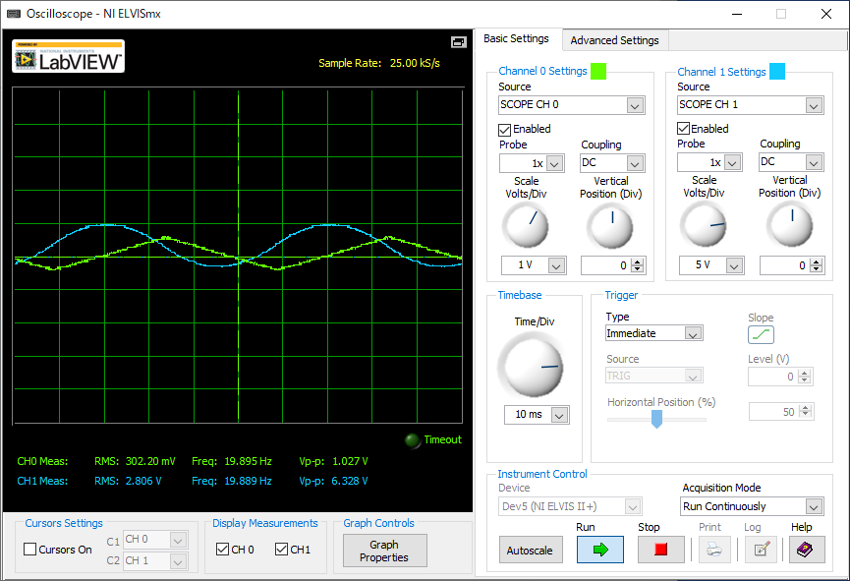
\includegraphics[width=0.8\linewidth]{src/figures/exp6/int-res-tri.png}
		\subcaption{不完全積分回路に三角波を入力したときの出力}\label{fig:exp6-int-res-tri}
	\end{subfigure}
	\begin{subfigure}{0.48\linewidth}
		\centering
		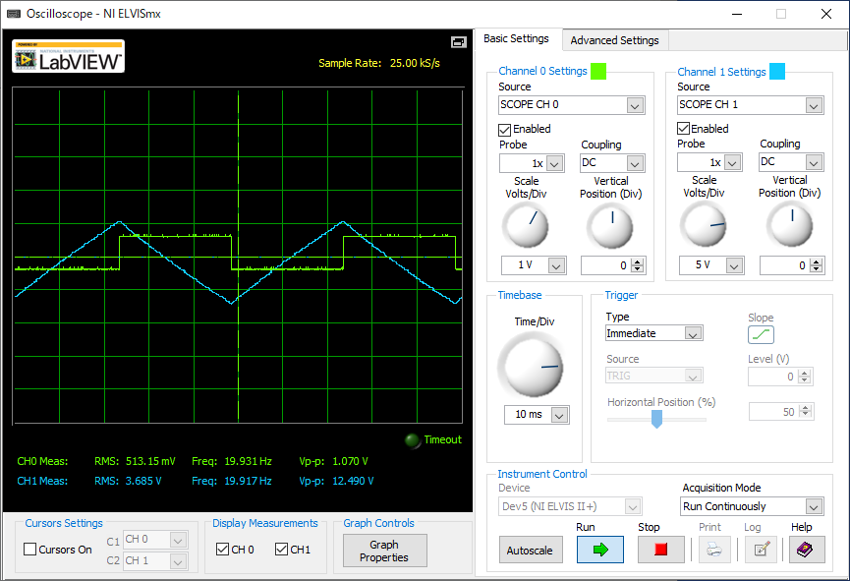
\includegraphics[width=0.8\linewidth]{src/figures/exp6/int-res-sq.png}
		\subcaption{不完全積分回路に矩形波を入力したときの出力}\label{fig:exp6-int-res-sq}
	\end{subfigure}
	\caption{実験6で撮影した画像}\label{fig:exp6-raw}
\end{figure}
